\section{Criterios de Selección}

Para identificar estas candidatas a variables cataclísmicas utilizamos el
catálogo de \hyperref[muestra:sec:gaia]{\gaia} para obtener una amplia muestra
fotométrica de estrellas dentro de la Galaxia. Gracias a la alta precisión y
sensibilidad de los instrumentos de \gaia es posible observar estrellas que no
han sido bien documentadas en la literatura. Para esto utilizamos la base de
datos dinámica de SIMBAD\footnote{\url{http://simbad.cds.unistra.fr/simbad/}}
para identificar estrellas cuya clasificación sea de interés para nuestra
investigación. Estas las priorizamos en base a la cantidad de datos disponibles
en la literatura; aquellos sistemas con la menor cantidad de referencias en la
literatura (obtenidas de SIMBAD) tienen una mayor prioridad que aquellos
objetos con varios estudios publicados.

\subsection{Búsqueda Fotométrica}

Para obtener la muestra inicial de objetos de interés acudimos a la base de datos de Gaia. Tal como es descrito en la sección \ref{muestra:sec:gaia} la selección de objetos fue llevada a cabo dentro del \textit{Gaia Archive} utilizando su interfaz de ADQL. Sin embargo, los criterios definidos por Szkody y colaboradores solo fueron definidos para el sistema fotométrico de SDSS; para poder utilizar estos primero se llevó a cabo una conversión de las magnitudes reportadas en el catálogo de Gaia a magnitudes en los pasa bandas de SDSS. Esta conversión se llevó a cabo utilizando las siguientes relaciones definidas en la documentación de Gaia DR3 \citet{gdr3ReleaseDocumentation}, tal como se puede ver en la figura \ref{gdr3SdssConversionGraphs}.

\begin{figure}[!h]
	\centering
	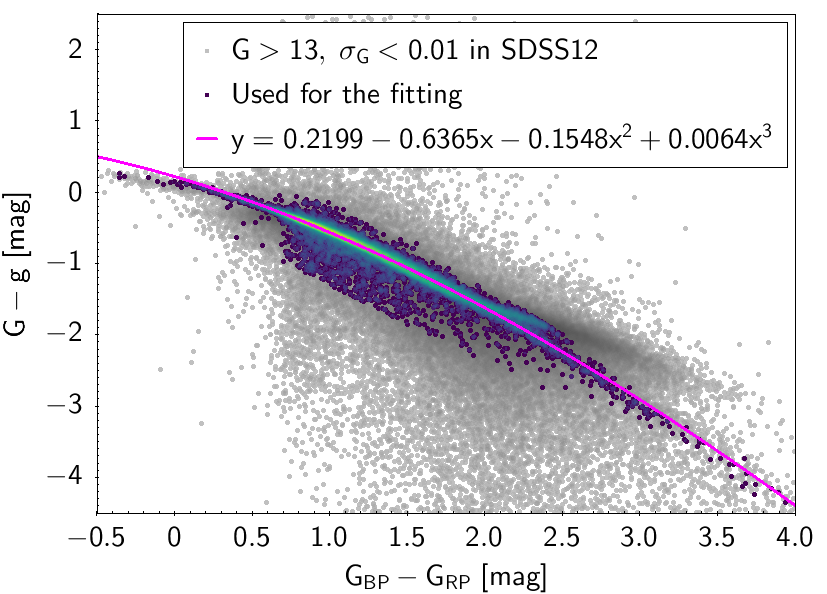
\includegraphics[scale=0.27]{Muestra/Secciones/Figures/Gaia-SDSS-Transform-g.png}
	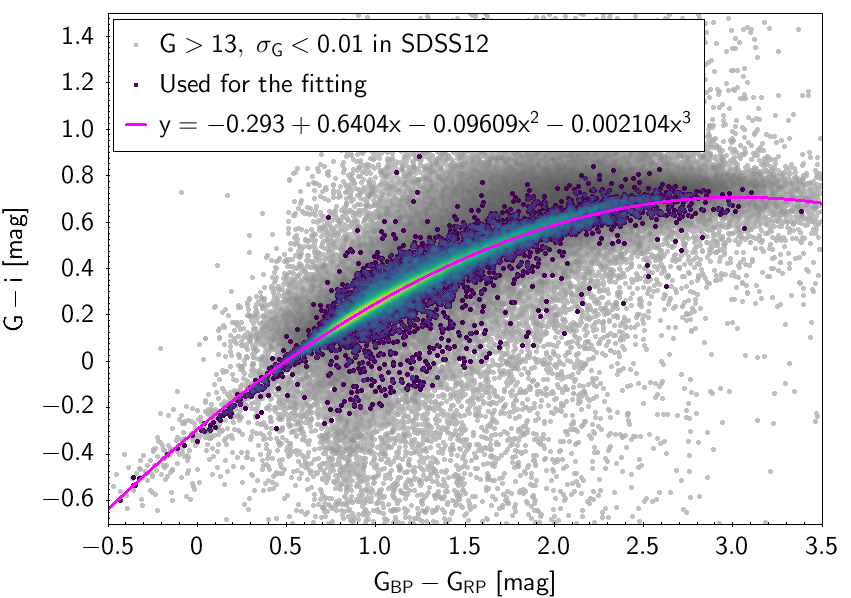
\includegraphics[scale=0.27]{Muestra/Secciones/Figures/Gaia-SDSS-Transform-i.png}
	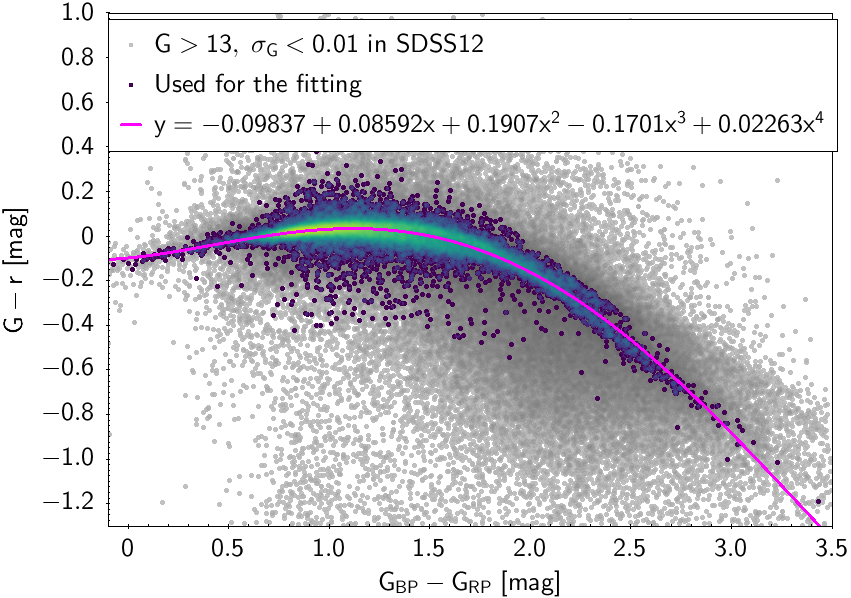
\includegraphics[scale=0.27]{Muestra/Secciones/Figures/Gaia-SDSS-Transform-r.png}

	\caption{Relación empírica }
	\label{gdr3SdssConversionGraphs}
\end{figure}